% 第五章 旋翼无人机目标检测定位系统

\chapter{旋翼无人机目标检测定位系统}

\section{旋翼无人机系统搭建}
\subsection{硬件系统集成}
在综合考虑了旋翼无人机的尺寸、载重能力、续航时间等因素,并比较了市场上可选择的双目摄像机和便携计算设备
产品后,本文在实验中搭建了以ZED双目摄像机为立体图像传感器、以英伟达Jetson TX2开发板为机载处理器、以Pixhawk为多旋翼飞行控制器、以组装六旋翼为飞行平台的旋翼无人机目标检测与定位系统,如图\ref{fig:5_1_旋翼无人机目标检测定位系统}所示。

\begin{figure}[htb] %旋翼无人机目标检测定位系统
	\centering
	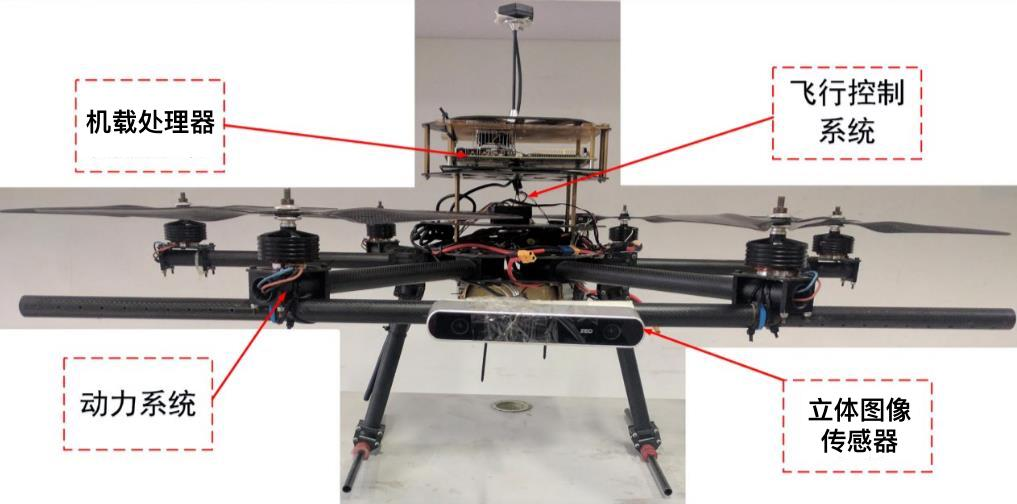
\includegraphics[width=6in]{figures/5_平台介绍/旋翼无人机目标检测定位系统}
	\caption{旋翼无人机目标检测定位系统}\label{fig:5_1_旋翼无人机目标检测定位系统}
\end{figure}

1、ZED双目立体相机

ZED是Stereolabs公司推出的双目立体相机。该相机获取的立体图像质量很高,因为其内部对左右两个摄像机进行了硬件同步,使用OpenCV对其进行操作时获取的是唯一的设备ID,每次从相机读取图片时获得的是左右视图拼接在一起的单幅图片,需要手动进行分割才能得到左右图像。ZED双目相机可以输出WVGA/720P/1080P/2K等多个分辨率的图片,由于使用了USB 3.0接口,当分辨率为720P时,输出帧率可达60fps,而当输出为2.2K的高分辨率图像时,仍能保持15fps的帧率。ZED相机具有较大的视角范围,最大水平视角可达110度。

Stereolabs为每一台出厂的相机提供了工业级的标定数据,可用来与摄像机标定实验的结果进行对比;还提供了一个强大的SDK,可以直接调用API来获取实时的具有较高精度的深度结果,深度范围为0.5-20m。另外还提供了修改相机参数(饱和度、对比度、亮度、曝光等)、6自由度的位置追踪、三维空间建图、SVO视频录制等功能。ZED SDK输出的深度图精度较高,但由于要检验本文的立体匹配算法,因此实验中仅使用OpenCV获取相机拍摄的原始图像,之后利用标定实验获得的参数进行立体校正,最后使用DispNetC模型获取深度结果。使用OpenCV配置相机时分辨率只有三个选择,实验中使用1280x720。ZED相机参数见表\ref{tab:5_ZED}。

\begin{table}[htb] %ZED双目立体相机参数
	\centering
	\caption{ZED双目立体相机参数}
	\label{tab:5_ZED}
	\begin{small}
%	\begin{tabular}{|c|c|}\hline
	\begin{tabular*}{\textwidth}{@{\extracolsep{\fill}}cc} \toprule[2pt]
		基线长度 & 12cm \\
		有效深度范围   & 0.5-20m \\
		分辨率@帧率 & 2208x1242@15/1080P@30/720P@60/672x376@100 \\
		视角范围 & 96° H, 54° V \\
		物理尺寸 & 175x30x33 mm \\
		重量 & 159g \\
		接口类型 & USB 3.0 \\
		供电 & 通过USB供电,5V/380mA \\
		兼容的操作系统 & Windows 7/8/10; Linux \\
		第三方支持 & ROS, unity, OpenCV, MATLAB \\ \bottomrule[2pt]
	\end{tabular*}
	\end{small}
\end{table}
%基线长度: 12cm
%有效深度范围: 0.5-20 m
%分辨率@帧率: 2208x1242@15/1920x1080@30/1280x720@60/672x376@100
%视角范围: 96° H, 54° V
%物理尺寸: 175x30x33 mm
%重量: 159g
%接口类型: USB 3.0
%供电: 通过USB供电,5V/380mA
%兼容的操作系统: Windows 7/8/10; Linux
%第三方支持: ROS, unity, OpenCV, MATLAB

%------------------------------------------------------------------------------------
2、NVIDIA Jetson TX2嵌入式平台

Jetson TX2是人工智能计算公司英伟达(NVIDIA)于2017年3月发布的一款嵌入式超级计算平台,被誉为“嵌入式领域的AI超级电脑”。其具有强大的计算能力,同时功耗和尺寸较小,因而非常适合应用于机器人、无人机、自动驾驶、智慧城市等领域。

Jetson TX2板载6核CPU处理器(4个Cortex-A57和2个Denver核心)和集成256个CUDA核心、基于Pascal架构的GPU,CPU和GPU共享8GB 128bit LPDDR4内存,内存带宽高达每秒58GB。最高支持连接6个摄像机,拍照带宽为2.5Gbps;对于4K分辨率的视频的编解码速度达到了60fps。数据存储使用高速的eMMC,存储空间为32G,另外支持外接SATA硬盘。开发板提供了丰富的外设接口,如CAN、UART、SPI、I2C等,非常便于与其他模块的交互。Jetson TX2较上一代产品TX1的计算性能提升了一倍,同时功耗比也提高了一倍,常规运行模态下功耗只有不到7.5W,直接通过一个稳压模块连接到旋翼无人机使用的同种电池上,即可解决开发板的供电问题。

开发板上运行的操作系统是基于aarch64架构的Ubuntu 16.04,因此在台式计算机上配置的开发环境和部署的代码都可以比较容易地移植到TX2上以应用于移动平台。此外,英伟达公司为Jetson系列开发板提供了JetPack软件开发工具包,包含面向GPU加速计算的CUDA工具箱、面向深度学习的深度神经网络库cuDNN和面向计算机视觉的OpenCV4Tegra等工具,大大方便了相关应用程序的开发。

\begin{figure}[htbp]
	\centering
	\begin{minipage}[c]{0.3\textwidth}
		\centering
		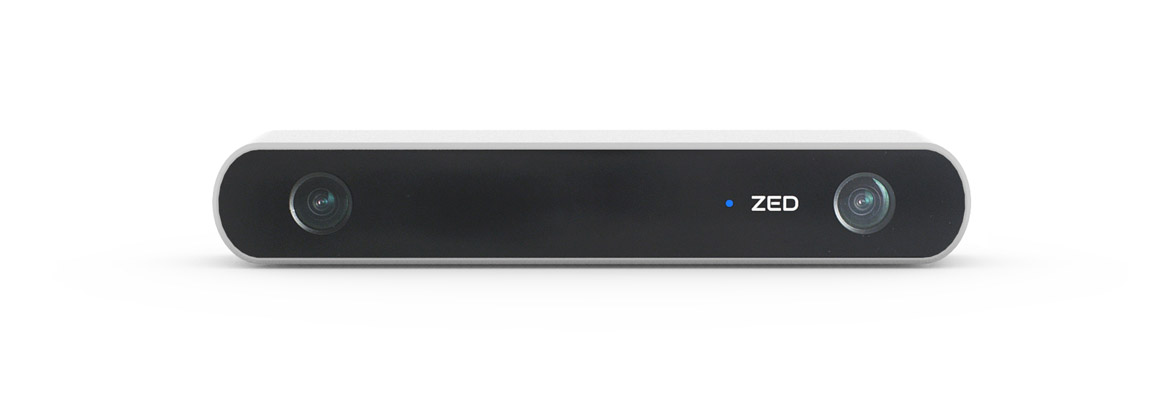
\includegraphics[width=2in]{figures/5_平台介绍/ZED}
		\caption{ZED双目立体相机}
	\end{minipage}
	\hfill
	\begin{minipage}[c]{0.3\textwidth}
		\centering
		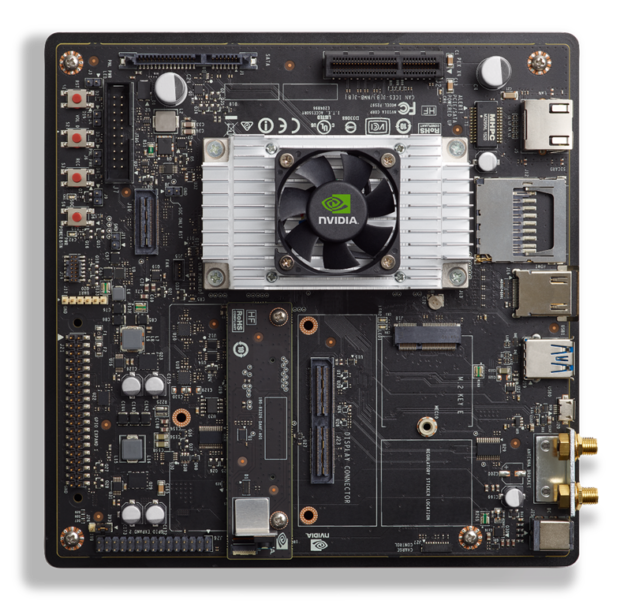
\includegraphics[width=1.5in]{figures/5_平台介绍/TX2}
		\caption{TX2开发板}
	\end{minipage}
	\begin{minipage}[c]{0.3\textwidth}
		\centering
		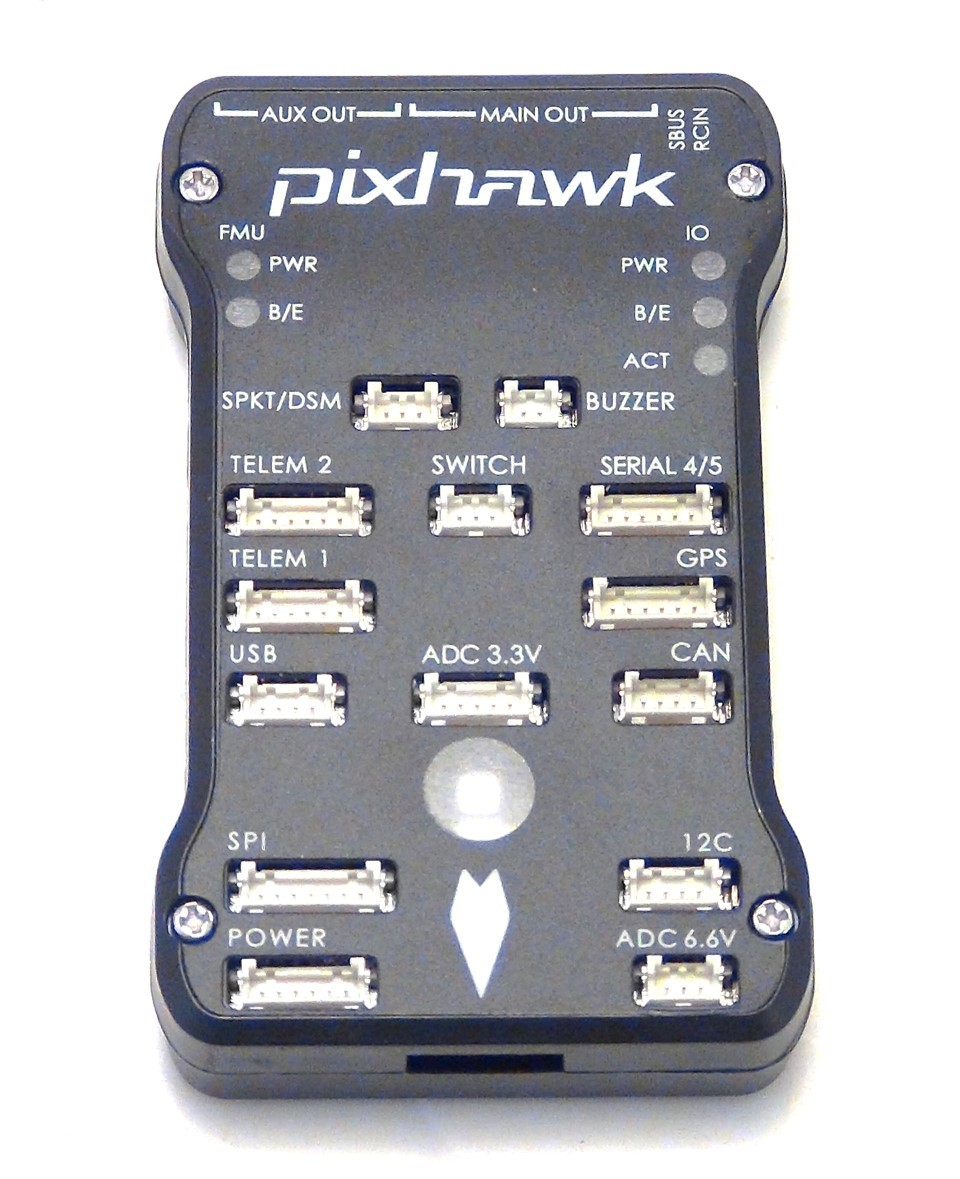
\includegraphics[width=1.2in]{figures/5_平台介绍/pixhawk}
		\caption{Pixhawk飞行控制器}
	\end{minipage}
\end{figure}

%------------------------------------------------------------------------------------
3、Pixhawk飞行控制器

Pixhawk是一款非常流行的开源自动驾驶控制器,可应用于固定翼、多旋翼等飞行器和智能车、船等移动机器人平台的控制。其由苏黎世联邦理工大学的实验室与3D Robotics和ArduPilot等团队合作设计而成,面向学术研究、个人爱好者和工业界,以较低的成本提供了很高的可用性。Pixhawk搭载了丰富的传感器,并提供了大量IO接口,能够满足应用开发需求;除了低成本高性能的STM32F4主处理器,还配备了一个协处理器用于失效保护,提高系统的可靠性。Pixhawk的具体硬件参数见表\ref{tab:5_Pixhawk}。
\begin{table}[htb] %Pixhawk硬件参数
	\centering
	\caption{Pixhawk硬件参数}
	\label{tab:5_Pixhawk}
	\begin{small}
%		\begin{tabular}{|c|c|}\hline
		\begin{tabular*}{\textwidth}{@{\extracolsep{\fill}}cc} \toprule[2pt]
			处理器 & 32位Arm Cortex M4主处理器(168Mhz/256KB RAM/2MB Flash),32位协处理器 \\
			传感器 & MPU6000等三轴加速度计、陀螺仪、磁罗盘;MS5611气压计 \\
			外设接口 & 5个UART串口,2个CAN,I2C,SPI,3.3/6.6V ADC,mini USB等 \\
			遥控输入 & Specktrum DSM/DSM2/DSM-X卫星输入,Futaba SBUS,PPM \\
			尺寸 & 长81.5mm,宽50mm,高15.5mm,重量38g \\
			其他 & 14路PWM输出;冗余的供电输入;外部安全开关、状态指示灯和蜂鸣器
			\\ \bottomrule[2pt]
		\end{tabular*}
	\end{small}
\end{table}


%------------------------------------------------------------------------------------
4、六旋翼无人机

由于需要挂载的机载处理器和双目摄像机重量较大,为了确保无人机具有足够的载荷能力,实验中自行组装了一台使用碳纤维材料机架、以无刷直流电机为动力的六旋翼飞行器。飞行器上的电机、电调、GPS、数传、遥控接收器等模块在此不做具体介绍。无人机空载时质量约为2kg,最大负载为5kg,使用6S 10000mAh的LiPo电池供电,续航时间约20分钟,可以满足实验需求。

%下一小节如果介绍软件系统集成,MissionPlanner就不要放在这。
此外,实验中使用运行Windows操作系统的联想笔记本电脑作为地面站,Mission Planner作为地面站软件,以进行起飞前的飞行控制相关参数设定、加速度计和磁罗盘等传感器的校准、飞行航线和任务规划,以及飞行中的状态监控。
地面站与遥控器共同组成地面控制系统,负责具体的飞行任务,确保飞行安全。

如图\ref{fig:5_1_数据链路}所示,整个系统中建立了ZED双目相机——Jetson TX2——Pixhawk——地面站的数据链路:ZED双目相机实时获取图像,通过USB传输给TX2开发板;TX2运行目标检测与立体匹配算法程序,计算出目标信息后通过串口通信发送给Pixhawk;最后Pixhawk利用数传将目标信息回传到地面站。

\begin{figure}[htb] %数据链路
	\centering
	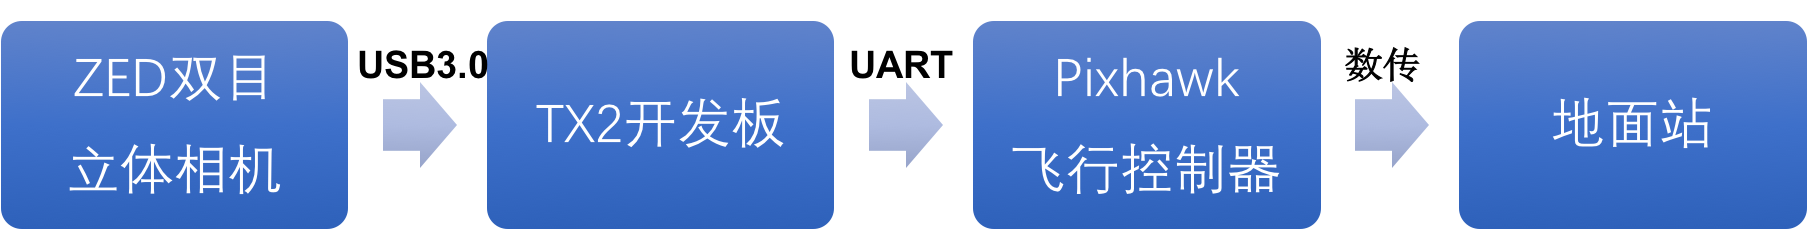
\includegraphics[width=6in]{figures/5_平台介绍/数据链路}
	\caption{数据链路}\label{fig:5_1_数据链路}
\end{figure}


\subsection{软件和算法系统集成}
本文第三、四章分别使用TensorFlow搭建了目标检测和立体匹配的卷积神经网络模型,需要在应用时将两个模块的结果进行融合以完成对目标的定位。此外,对于立体匹配模块,网络的输入需为立体校正后的图像,因此需要先对ZED拍摄的立体图像进行处理。考虑到基于TensorFlow的主体算法部分是使用Python语言实现的,为了尽量保持系统内的一致性,我们使用开源计算机视觉函数库OpenCV的Python接口(即cv2模块)进行图像的获取、立体校正和其他预处理操作。在融合目标检测和立体匹配的结果得到摄像机坐标系下目标的三维坐标后,可使用pyserial模块进行串口通信。

飞行控制器Pixhawk上运行的是开源飞行控制软件ArduPilot。ArduPilot使用C++开发,支持固定翼飞行器、多旋翼飞行器和车辆等多种模型,对应多旋翼飞行器的软件模块为ArduCopter。由于使用了硬件抽象层机制,其可以运行于多个硬件平台上。目标在摄像机坐标系下的三维坐标转化到机体或世界坐标系下时需要利用飞行器的姿态与位置信息,因此坐标变换可采用两种方案:飞行控制器将惯性导航系统获得的姿态与位置信息通过串口发送给TX2,在TX2上完成坐标变换后发回给飞行控制器,或飞行控制器直接进行计算。由于坐标变换的计算量不大,且最终与地面站的通信是通过飞控的数传完成的,因此在ArduPilot中添加坐标变换的相关代码效率更高。
飞控与地面站的通信使用Mavlink通信协议。

综上所述,可以作出整个目标检测定位系统的算法集成示意图,如图\ref{fig:5_1_算法集成示意图}所示。图中坐标变换之前的部分全部在Jetson TX2开发板上执行,坐标变换和最后的通信由飞行控制器Pixhawk负责。

\begin{figure}[htb] %算法集成示意图
	\centering
	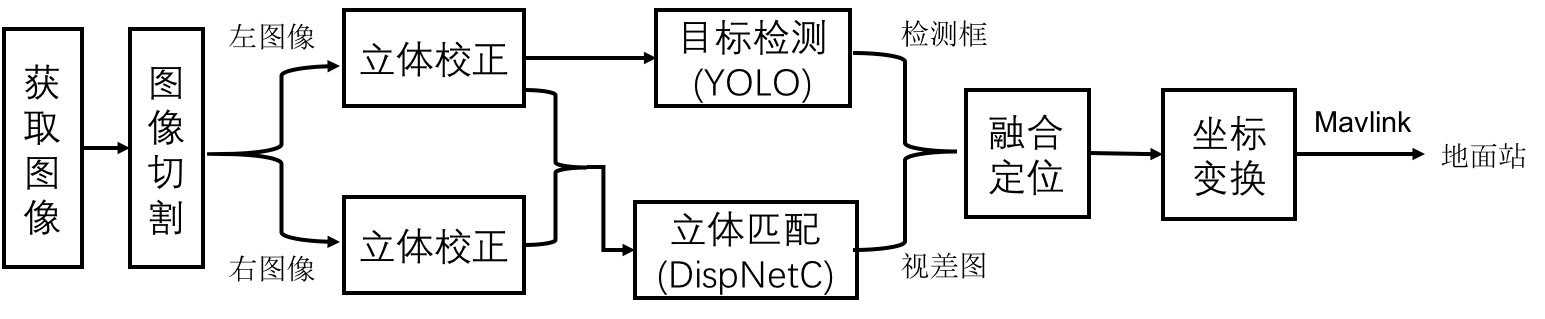
\includegraphics[width=6in]{figures/5_平台介绍/算法集成示意图}
	\caption{算法集成示意图}\label{fig:5_1_算法集成示意图}
\end{figure}

%------------------------------------------------------------------------------------
\section{目标定位}
% 第二章立体校正最后的重投影矩阵Q,《学习opencv》P503.
在使用YOLO网络模型完成了目标检测的任务后,对于每个目标,我们得到了一个将其包含在内的检测框;另一方面,利用DispNetC网络模型,我们得到了整张图片的视差图,也就获得了图像中任意像素点对应三维空间中的点的深度信息。只需要在检测框中确定对应目标中心位置的像素点,就可以根据双目立体视觉理论计算得到目标在摄像机坐标系下的三维坐标。再进行相应的坐标变换操作,即可完成目标在所需坐标系下的定位任务。

% 两个系统融合的框图

\subsection{图像坐标系下目标中心的确定}
%给两个方案:grabcut和直接取bbox中心,根据应用要求来选。
目标检测算法对每个目标返回一个矩形框,要确定目标中心在图像中的位置,最简单的方法是直接选取矩形框的中心。然而,由于目标检测算法的精度、摄像机拍摄时的姿态与目标形状等因素的影响,这种简单的方法并不能保证所定位的目标中心的准确性。因此,本文使用图像分割算法GrabCut来提取目标的轮廓,之后在轮廓范围内进行中心坐标的计算。

% 《基于双目立体视觉的目标识别与抓取定位》,王德海。ch4.1, p52.
% http://blog.sina.com.cn/s/blog_1584387c90102x5fu.html
% http://blog.csdn.net/peaceinmind/article/details/50135081
GrabCut算法\cite{rother2004grabcut}是一种基于图割(Graph Cuts)\cite{boykov2001interactive}的交互式图像分割算法。图割作为一种能量优化算法,被广泛地应用于图像分割、立体视觉、抠图等领域。在图像分割中,其将图像表示为一个无向图,每个像素作为图中的一个节点,在图中添加两个节点s和t分别代表前景和背景,在相邻像素点之间、每个像素与s/t节点之间建立边。然后构造一个能量函数,区域项由每个像素属于前景和背景的概率决定,边界项由相邻像素之间的相似程度决定,从而把图像分割问题转化为一个无向图的最小割问题。

\begin{figure}[htb] %Graph Cuts示意图
	\centering
	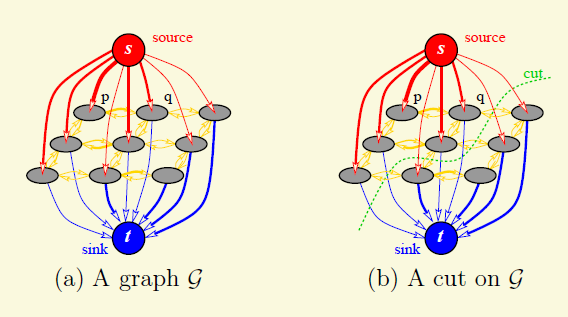
\includegraphics[width=4in]{figures/5_2_graphcuts}
	\caption{Graph Cuts示意图}\label{fig:5_1_Graph Cuts示意图}
\end{figure}

GrabCut对Graph Cuts算法做了一些改进,使用高斯混合模型(GMM)代替灰度直方图来分别对前景和背景进行建模,从而可以支持对彩色图像的分割;模型参数的学习是通过迭代方式进行的,而不是对能量函数进行一次性最小化;只需提供背景区域的像素集,不再需要分别指定目标和背景中的种子点。

%opencv grabcut函数介绍。
具体地,GrabCut需要用户提供一个矩形框,矩形框外的区域确定为背景,矩形框内包含前景,同时也包含部分背景。目标检测得到的检测框恰好可以用来作为这个矩形框。有时目标检测得到的检测框可能不准确,因此可以设定一个阈值,将检测框向外扩大一定的范围再传入GrabCut算法。
分割结束后会得到一个掩码矩阵mask,根据其中的元素值即可确定每个点是否属于前景。使用下式计算前景区域内像素坐标平均值,作为图像中的目标中心:
\begin{equation}
\left\{
\begin{array}{l}
\bar{u} = \frac{1}{m}\sum\limits_{i=1}^{m}u_i \\
\bar{v} = \frac{1}{m}\sum\limits_{i=1}^{m}v_i \\
\end{array}
\right.
\end{equation}
其中,$(\bar{u}, \bar{v})$为目标中心坐标,$(u_i, v_i)$为第i个像素点的坐标,m为分割结果中前景区域内的像素点数量。


GrabCut有一定的时间消耗,因此应该根据应用的实时性要求来选择确定目标中心的方法。当实时性要求高时,直接使用目标检测框的中心作为近似的目标中心;当目标为静止目标、对实时性没有严格要求时,首先使用GrabCut算法提取目标轮廓,以获得更精确的目标中心位置。

\subsection{补充坐标系定义及变换} %云台要不要?不想要
第二章中介绍了图像与摄像机相关的坐标系。由于要将双目摄像机挂载在旋翼无人机上,在此对无人机的控制与导航系统使用的坐标系进行补充。

1、机体坐标系$O_b-x_by_bz_b$

机体坐标系固连在飞行器上,原点位于其质心处。$x_b$轴位于无人机的对称平面内,水平指向前方;$y_b$轴垂直于无人机的对称平面,指向右方;$z_b$轴沿对称平面内与x轴垂直指向下方。

2、导航坐标系$O_n-x_ny_nz_n$

导航坐标系又称为地理坐标系,实际上与前面定义的世界坐标系的概念是类似的,但在定义世界坐标系时并未规定各坐标轴的方向,故在此明确为“北-东-地”(NED)坐标系。选定地球表面某一点作为坐标系原点,$x_n$轴由原点水平指向北,$y_n$轴水平指向东,$z_n$轴垂直于地面指向下方。

无人机的姿态,即机体坐标系与导航坐标系之间的关系,一般使用三个欧拉角来描述。机体坐标系的$x_b$在水平面$x_n O y_n$内的投影与导航坐标系的$x_n$轴之间的夹角被称为偏航角(yaw angle, $\psi$);机体坐标系的$x_b$轴与水平面$x_n O y_n$之间的夹角被称为俯仰角(pitch angle, $\theta$);机体轴$z_b$与$x_b$轴所在的铅垂面之间的夹角被称为滚转角(roll angle, $\phi$)。偏航角取值范围为$[0^{\circ}, 360^{\circ}]$,右偏航为正;俯仰角和滚转角的取值范围为$(-90^{\circ}, 90^{\circ})$,无人机抬头时俯仰角为正,向右滚转时滚转角为正。

机体坐标系与导航坐标系之间的转换可使用旋转矩阵(也叫方向余弦矩阵)来完成。由于旋转不具有交换性,因此由导航坐标系变换到机体坐标系需严格按照偏航角$\rightarrow$俯仰角$\rightarrow$滚转角的顺序依次进行旋转。首先绕$z_n$轴转动偏航角的旋转矩阵为:
%
\begin{eqnarray}
C_\psi =
\begin{bmatrix}
cos\psi & sin\psi & 0 \\
-sin\psi & cos\psi & 0 \\
0 & 0 & 1
\end{bmatrix}
\end{eqnarray}

其次,绕$y_n$轴转动俯仰角的旋转矩阵为:
%
\begin{eqnarray}
C_\theta =
\begin{bmatrix}
cos\theta & 0 & -sin\theta \\
0 & 1 & 0 \\
sin\theta & 0 & cos\theta
\end{bmatrix}
\end{eqnarray}

最后,绕$x_n$轴旋转滚转角的旋转矩阵为:
%
\begin{eqnarray}
C_\phi =
\begin{bmatrix}
1 & 0 & 0 \\
0 & cos\phi & sin\phi \\
0 & -sin\phi & cos\phi \\
\end{bmatrix}
\end{eqnarray}

将三个旋转矩阵结合,即可得到由导航坐标系到机体坐标系的旋转矩阵:
%
\begin{eqnarray}
C_n^b = C_\phi C_\theta C_\psi =
\begin{bmatrix}
cos\theta cos\psi & cos\theta sin\psi & -sin\theta \\
sin\theta cos\psi sin\phi - sin\psi cos\phi & sin\theta sin\psi sin\phi + cos\psi cos\phi & cos\theta sin\phi \\
sin\theta cos\psi cos\phi + sin\psi sin\phi & sin\theta sin\psi cos\phi - cos\psi sin\phi & cos\theta cos\phi
\end{bmatrix}
\end{eqnarray}

旋转矩阵为正交矩阵,从而直接可以得到由机体坐标系到导航坐标系的旋转矩阵:
%
\begin{eqnarray}
C_b^n = (C_n^b)^{-1} = (C_n^b)^T
%\begin{bmatrix}
%cos\theta cos\psi & sin\theta cos\psi sin\phi - sin\psi cos\phi & sin\theta cos\psi cos\phi + sin\psi sin\phi \\
%cos\theta sin\psi & sin\theta sin\psi sin\phi + cos\psi cos\phi & sin\theta sin\psi cos\phi - cos\psi sin\phi \\
%-sin\theta & cos\theta sin\phi & cos\theta cos\phi
%\end{bmatrix}
\end{eqnarray}

%  云台:《旋翼无人机跟踪地面移动目标的视觉控制》[D],姜运宇,P17.
另外,摄像机坐标系与机体坐标系之间也需要进行转换。考虑一般情况,相机通过云台安装在无人机上,云台具有两个旋转自由度。由于云台安装位置与无人机质心之间的距离一般应远小于无人机与目标之间的距离,因此近似认为摄像机坐标系的原点与机体坐标系的原点重合。则机体坐标系与摄像机坐标系的关系如图\ref{fig:5_2_机体坐标系与摄像机坐标系的关系}所示。

\begin{figure}[htb] %机体坐标系与摄像机坐标系的关系
	\centering
	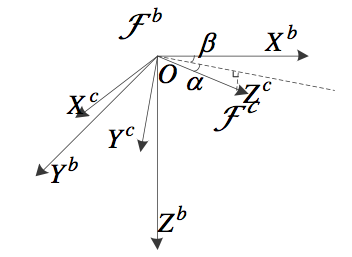
\includegraphics[width=3in]{figures/5_2_机体坐标系与摄像机坐标系之间的关系}
	\caption{机体坐标系与摄像机坐标系的关系}\label{fig:5_2_机体坐标系与摄像机坐标系的关系}
\end{figure}
$\alpha$和$\beta$分别表示云台的方向角和俯仰角。从而,由机体坐标系到摄像机坐标系的旋转矩阵为\cite{姜运宇2014旋翼无人机跟踪地面移动目标的视觉控制}:
%
\begin{eqnarray}
C_b^c =
\begin{bmatrix}
-sin\beta & cos\beta & 0 \\
sin\alpha cos\beta & sin\alpha sin\beta & cos\alpha \\
cos\alpha cos\beta & cos\alpha sin\beta & -sin\alpha
\end{bmatrix}
\end{eqnarray}

由于本文实验搭建的旋翼无人机目标检测定位系统中ZED双目立体相机是直接固定在机身上的,相当于云台的方向角$\alpha$和俯仰角$\beta$都为0,因此转换矩阵简化为:
%
\begin{eqnarray}
C_b^c =
\begin{bmatrix}
0 & 1 & 0 \\
0 & 0 & 1 \\
1 & 0 & 0
\end{bmatrix}
\end{eqnarray}
由相机坐标系到机体坐标系的转换矩阵$C_c^b = (C_b^c)^{-1} = (C_b^c)^T$。

\subsection{各个坐标系下的目标定位}
在确定了目标中心在图像中的坐标(u, v)及对应视差值d后,可以直接利用三角测量原理计算目标在摄像机坐标系下的坐标。第二章中使用立体校正函数stereoRectify()得到了图像坐标系到摄像机坐标系的重投影矩阵Q,有
%
\begin{eqnarray}
\begin{bmatrix}
X \\ Y \\ Z \\ W
\end{bmatrix}
= Q
\begin{bmatrix}
u \\ v \\ d \\ 1
\end{bmatrix}
\end{eqnarray}
从而目标在摄像机坐标系下的三维坐标$(X_c, Y_c, Z_c)$ = (X/W, Y/W, Z/W)。

之后可使用坐标变换计算目标在机体坐标系下的坐标。由于忽略了摄像机坐标系与机体坐标系原点间的距离,因此只使用旋转矩阵即可得到
%
\begin{eqnarray}
\begin{bmatrix}
X_b \\ Y_b \\ Z_b
\end{bmatrix}
= C_c^b
\begin{bmatrix}
X_c \\ Y_c \\ Z_c
\end{bmatrix}
\end{eqnarray}

最后计算目标在导航坐标系下的坐标时,除了进行旋转变换,还要从旋翼无人机的惯性导航系统中读取无人机当前相对于导航坐标系原点的坐标$(X_0, Y_0, -H)$作为平移向量加入结果中:
%
\begin{eqnarray}
\begin{bmatrix}
X_n \\ Y_n \\ Z_n
\end{bmatrix}
= C_b^n
\begin{bmatrix}
X_b \\ Y_b \\ Z_b
\end{bmatrix}
+
\begin{bmatrix}
X_0 \\ Y_0 \\ -H
\end{bmatrix}
\end{eqnarray}
将结果发送回地面站时,也可以选择将惯性坐标系下的坐标转换为GPS坐标,在此不再具体介绍。最后给出完整的目标定位系统流程图,如图\ref{fig:5_2_目标定位系统流程图}。

\begin{figure}[htb] %目标定位系统流程图
	\centering
	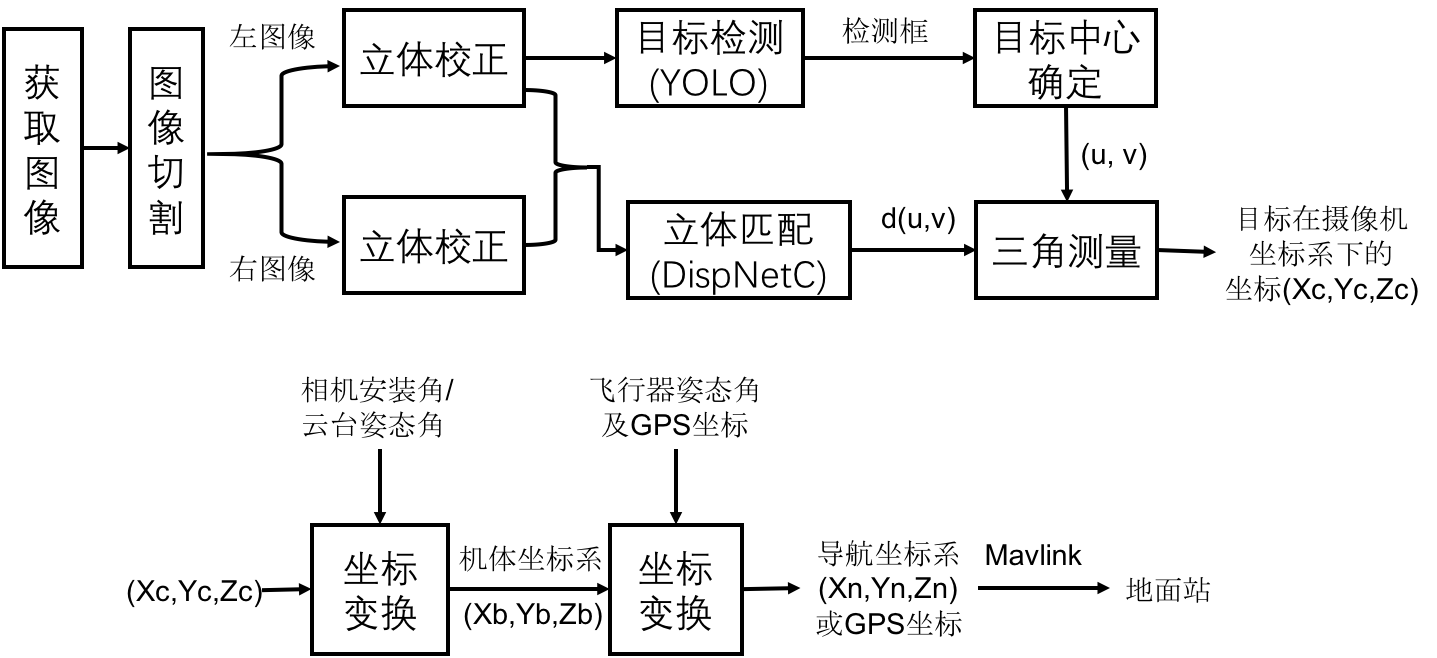
\includegraphics[width=6in]{figures/5_2_目标定位系统流程图}
	\caption{目标定位系统流程图}\label{fig:5_2_目标定位系统流程图}
\end{figure}

%------------------------------------------------------------------------------------
\newpage
\section{实验结果}
在此对照整个算法系统流程,详细地给出每个步骤的实验结果。首先,使用OpenCV的imread()函数获取ZED拍摄的图像并进行切割,得到左右图像,如图\ref{fig:5_3_原始图像}所示。可以明显看出图像受到相机畸变的影响,地面发生了严重的扭曲。显然这样的图像是无法用于立体匹配的。
\begin{figure}[htb] %原始图像
	\centering
	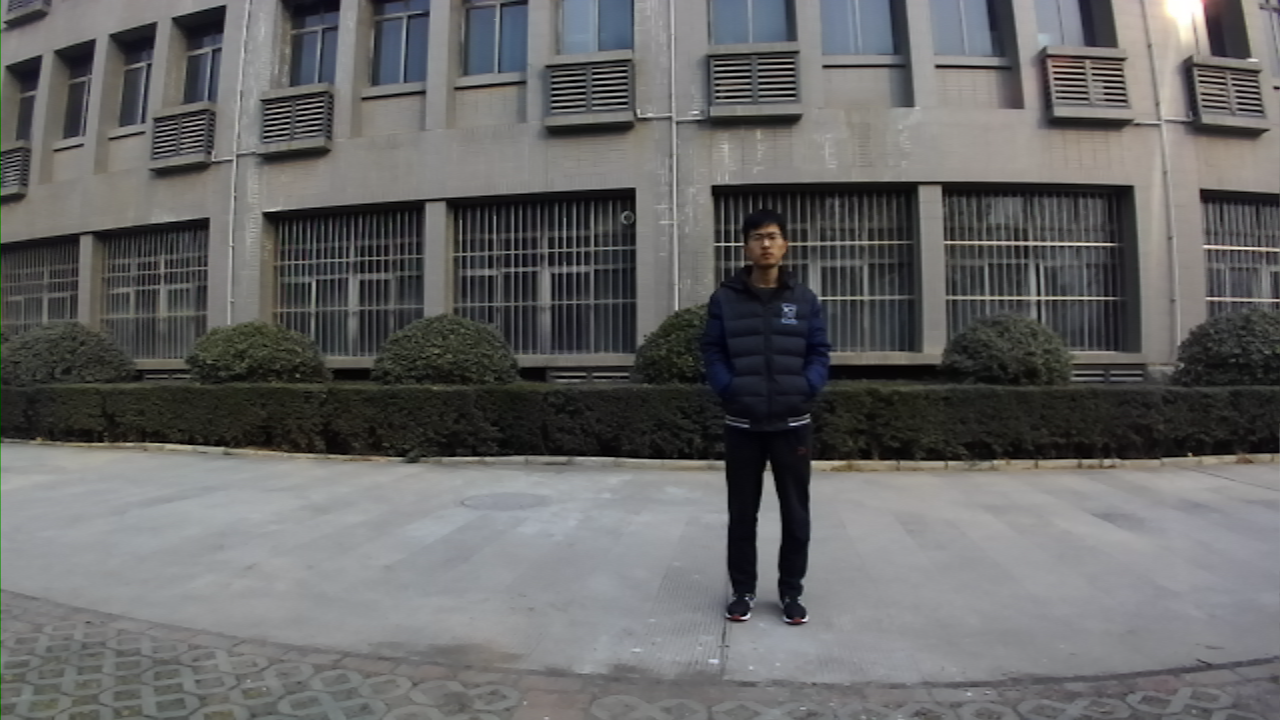
\includegraphics[width=3in]{figures/5_实验结果/left_7_raw}
	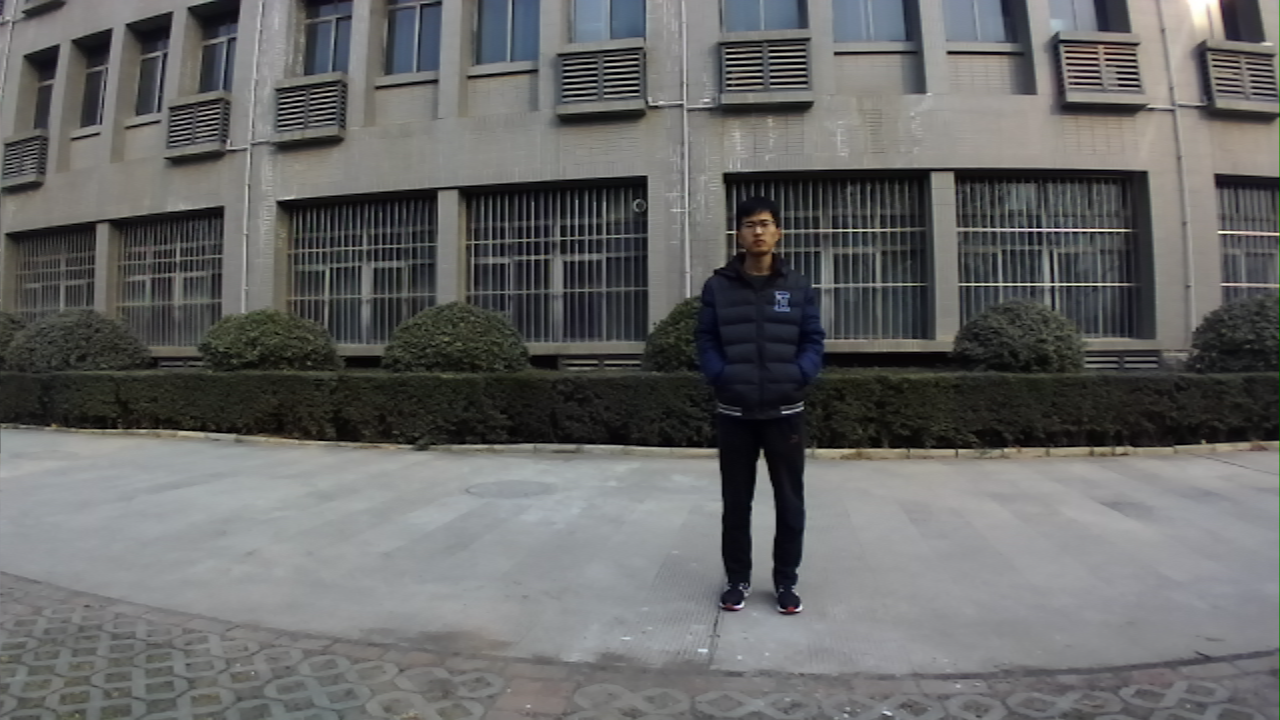
\includegraphics[width=3in]{figures/5_实验结果/right_7_raw}
	\caption{原始图像}\label{fig:5_3_原始图像}
\end{figure}

使用OpenCV的stereoRectify()函数进行立体校正,得到Rl、Rr、Pl、Pr四个矩阵,然后利用InitUndistortRectifyMap()函数计算校正前后图像的逐像素映射关系矩阵。之后就可以使用remap()函数通过查表操作来实现高效的立体校正。校正结果如图\ref{fig:5_3_立体校正结果}所示,原始图像中地面上扭曲的直线已经恢复正常。
\begin{figure}[htb] %立体校正结果
	\centering
	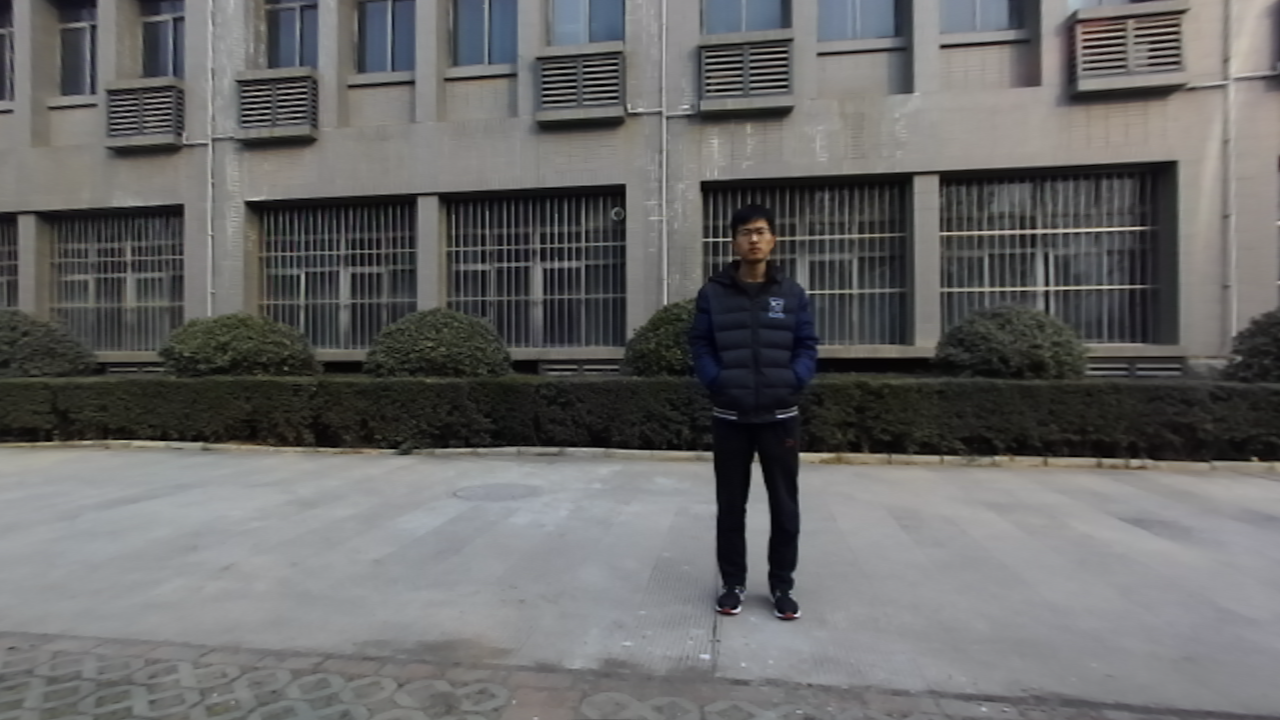
\includegraphics[width=3in]{figures/5_实验结果/left_7_rect}
	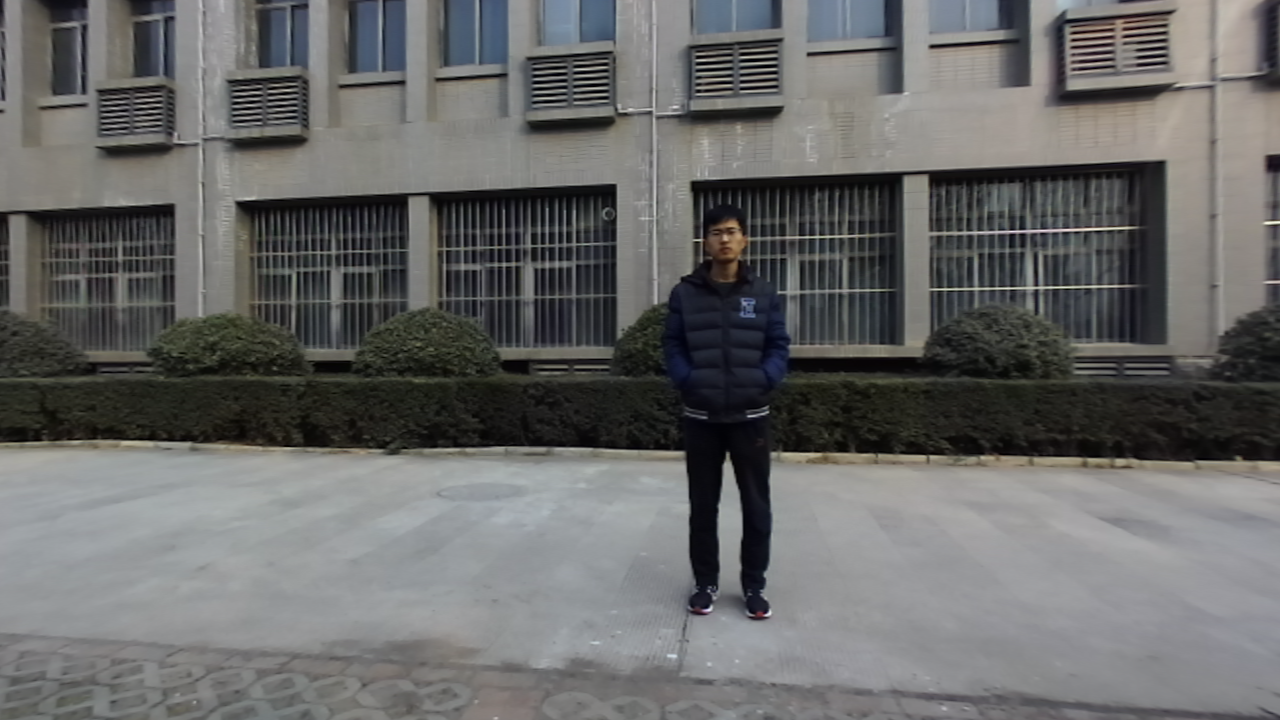
\includegraphics[width=3in]{figures/5_实验结果/right_7_rect}
	\caption{立体校正结果}\label{fig:5_3_立体校正结果}
\end{figure}

下一步,将左图输入YOLO目标检测系统,输出目标检测结果如图\ref{fig:5_3_目标检测结果};将左右图同时输入DispNetC网络进行立体匹配,得到与左图对应的视差图,如图\ref{fig:5_3_立体匹配结果}。目标检测的结果较为理想,上下边界准确地定位到了图像中人物的头顶与脚下,左右边界略宽,但并没有偏离,目标基本位于检测框的正中央。检测框的左上角和右下角的顶点坐标分别为(665, 212)和(859,621)。
立体匹配的结果不太明显,但可以看出图中人物的大致轮廓。这主要是由于ZED双目相机的基线较短,只有12厘米,匹配结果中最大的视差也只有40左右。
\begin{figure}[htb] %目标检测结果,立体匹配结果
	\centering
	\begin{minipage}[c]{0.48\textwidth}
		\centering
		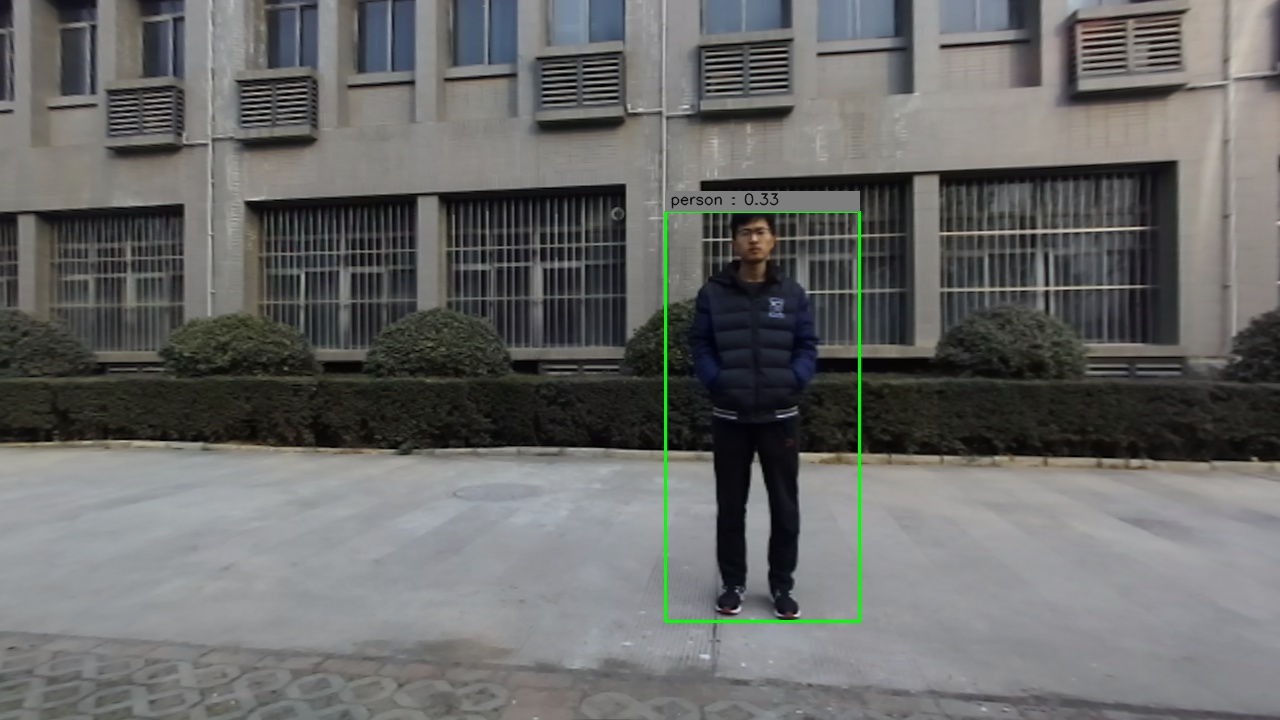
\includegraphics[width=3in]{figures/5_实验结果/left_7_detection}
		\caption{YOLO目标检测结果}\label{fig:5_3_目标检测结果}
	\end{minipage}
	\hfill
	\begin{minipage}[c]{0.48\textwidth}
		\centering
		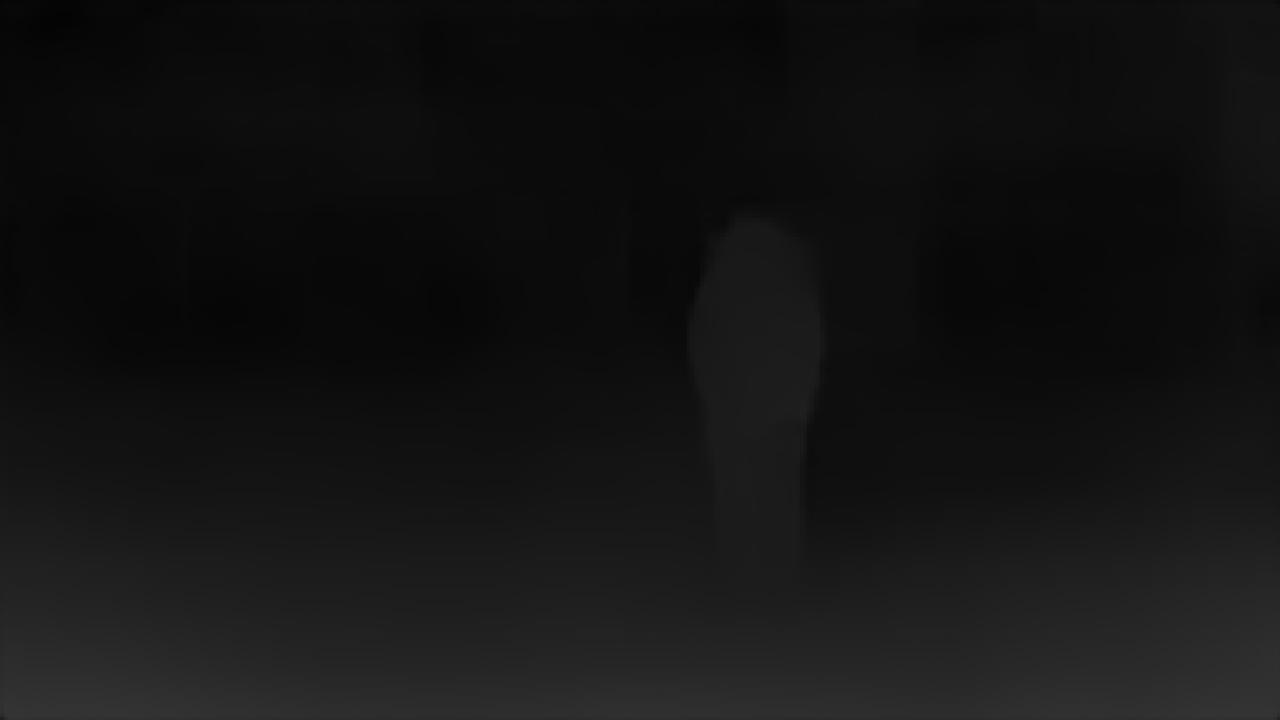
\includegraphics[width=3in]{figures/5_实验结果/disparity}
		\caption{DispNetC立体匹配结果}\label{fig:5_3_立体匹配结果}
	\end{minipage}
\end{figure}

之后,使用OpenCV的grabCut()函数进行图像分割,提取检测框内目标的轮廓。实验中分别对RGB图像和视差图进行了分割,最终得到的目标轮廓如图\ref{fig:5_3_RGB分割结果}和\ref{fig:5_3_视差图分割结果}所示。在RGB图像上进行分割获得的目标轮廓比视差图上的结果更加准确。由于人物的脚部与地面的深度是连续变化的,因此难以在视差图中将二者分开。
\begin{figure}[htb] %目标检测结果,立体匹配结果
	\centering
	\begin{minipage}[c]{0.48\textwidth}
		\centering
		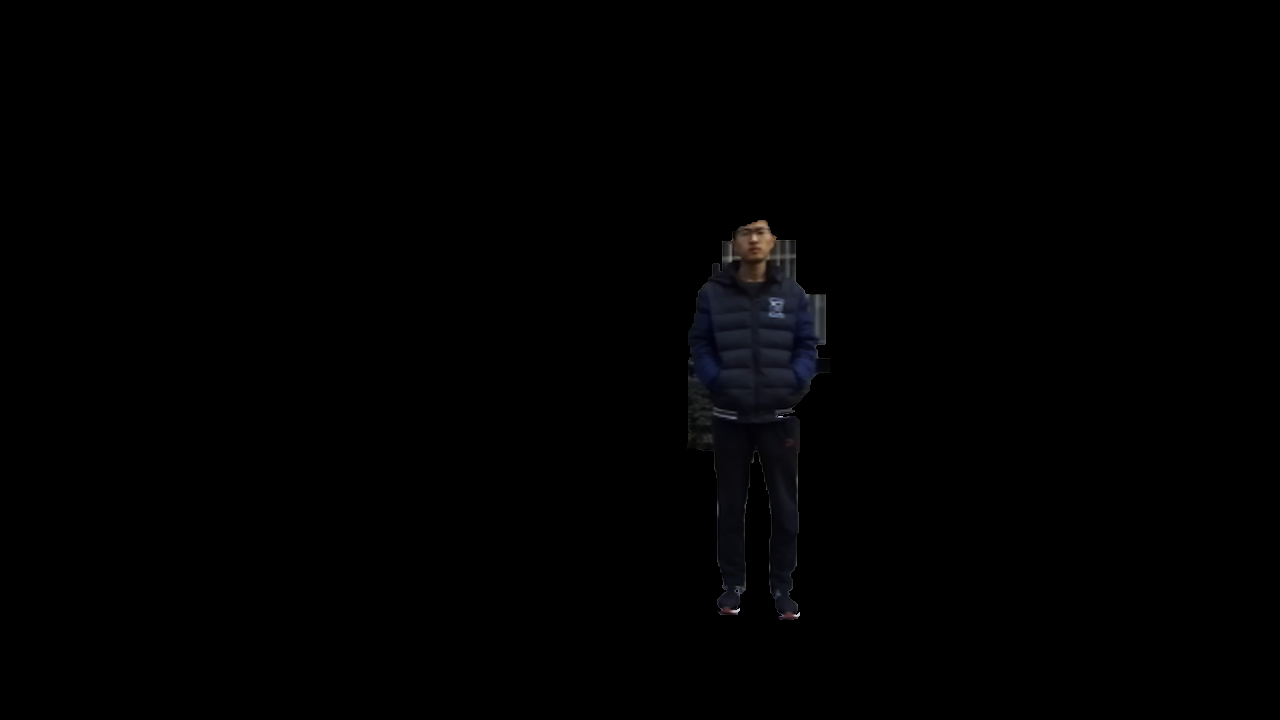
\includegraphics[width=3in]{figures/5_实验结果/rgb_seg/left_seg5}
		\caption{RGB图像分割结果}\label{fig:5_3_RGB分割结果}
	\end{minipage}
	\hfill
	\begin{minipage}[c]{0.48\textwidth}
		\centering
		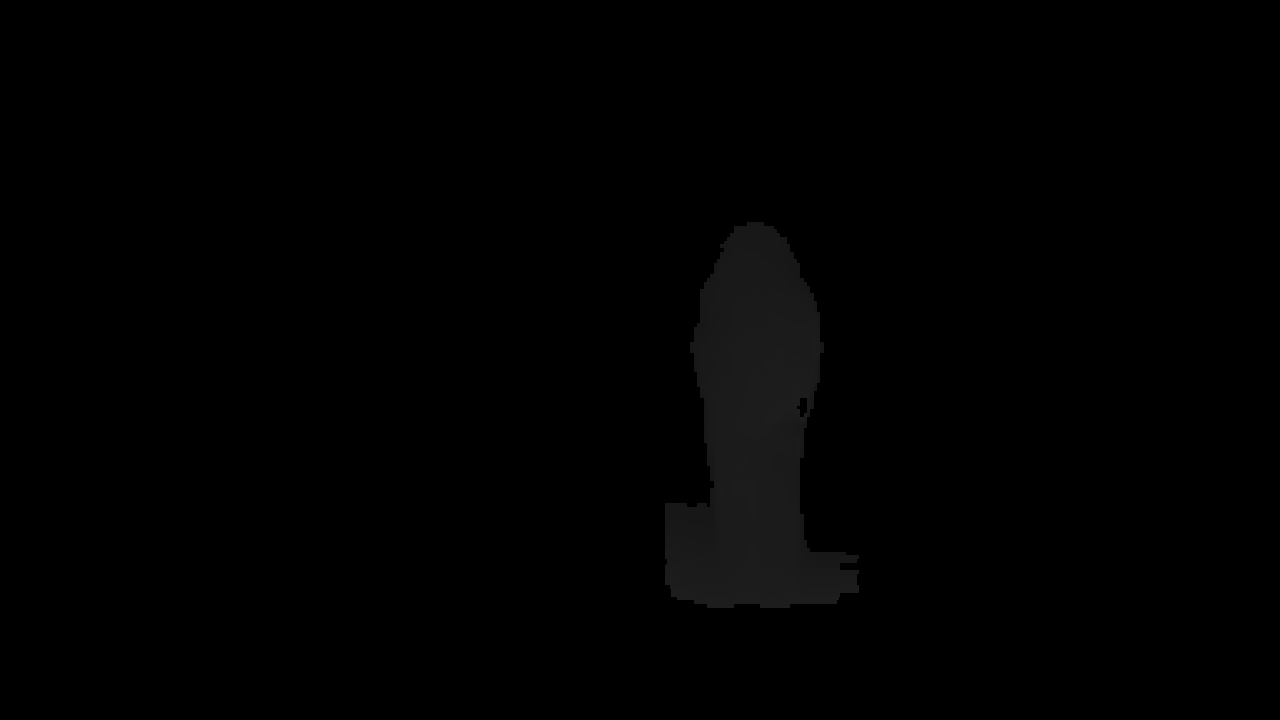
\includegraphics[width=3in]{figures/5_实验结果/disparity_seg/disp_seg5}
		\caption{视差图分割结果}\label{fig:5_3_视差图分割结果}
	\end{minipage}
\end{figure}

计算分割结果中前景像素点的坐标平均值,对应RGB图像和视差图的结果分别为(754, 395)和(754, 434)。检测框的中心坐标为(762, 417)。以分割RGB图像得到的结果(754, 395)作为目标中心坐标,视差图中该位置的像素值为28,即目标中心的视差d=28。利用图像坐标系到摄像机坐标系的重投影矩阵Q,可计算
%
\begin{eqnarray}
\begin{pmatrix} X \\ Y \\ Z \\ W \end{pmatrix}=
\mathbf{Q} \begin{pmatrix} u \\ v \\ d \\ 1 \end{pmatrix}
= \begin{pmatrix} 154.51 \\ 39.27 \\ 682.57 \\ 0.23296 \end{pmatrix}
\end{eqnarray}

从而,目标在摄像机坐标系下的三维坐标为(X/W, Y/W, Z/W) = (663.25, 168.57, 2929.99)mm,计算得到摄像机坐标原点到目标中心的距离为3.01米。拍摄图片时使用手持式激光测距仪测得的真实距离为3米,但由于测量时无法准确确定摄像机光心和目标中心,测得的距离也难免存在误差,因此保守估计误差小于3\%。对于距离更远的目标,实验中测试了10m左右距离的目标,误差约为10\%,由于其视差图中像素值都很小,因此未在文中给出。事实上,实验中的定位精度主要受到了ZED双目相机基线长度的制约。根据三角测量原理,深度与基线长度成正比,与视差成反比,因此立体视觉系统仅在有限的距离内具有较高的精度。结合实验中使用的相机的具体参数,可知深度与视差大致满足Z=82039.66/d的关系。做出视差与深度的对应关系表格如下。由表中可见,10米距离对应的视差为8,当视差变化1,深度的变化已经超过了1米,因此即使立体匹配的结果是准确的,仅因视差的不连续性导致的误差就可达到5\%,而如果立体匹配的结果有误差,最终得到的距离误差会更大。使用更长基线的双目相机,是提高目标定位有效范围和精度的直接途径。

\begin{table}[htb] %ZED相机视差与深度的对应关系
	\centering
	\caption{ZED相机视差与深度的对应关系}
	\label{tab:5_ZED相机视差与深度的对应关系}
	\begin{small}
%		\begin{tabular}{|cc|cc|cc|}\hline
		\begin{tabular*}{\textwidth}{@{\extracolsep{\fill}}cccccc} \toprule[2pt]
			视差d & 深度Z(mm) & 视差d & 深度Z(mm) & 视差d & 深度Z(mm) \\ \midrule[1pt]
			50      & 1641          & 12      & 6836         & 6        & 13673 \\
			40      & 2051         & 11       & 7458         & 5        & 16408 \\
			30      & 2735         & 10       & 8204        & 4        & 20510 \\
			25      & 3282         & 9        & 9115         & 3        & 27346 \\
			20      & 4102         & 8        & 10255       & 2        & 41019 \\
			15      & 5469         & 7        & 11720        & 1         & 82040 \\
			\bottomrule[2pt]
		\end{tabular*}
	\end{small}
\end{table}


%------------------------------------------------------------------------------------
%\section{应用讨论?}
%\subsection{飞行控制架构}
%\subsection{智能跟随}
%\subsection{自主避障}

%------------------------------------------------------------------------------------
\section{本章小结}
本章搭建了旋翼无人机目标检测定位系统。首先介绍了硬件系统的组成,包括ZED双目立体相机、英伟达Jetson TX2开发板、Pixhawk飞行控制器和六旋翼无人机等。之后给出了集成目标检测和立体匹配模块进行目标定位的思路,利用GrabCut算法对检测结果进行分割,从而确定出图像坐标系下目标中心坐标,结合立体匹配得到的视差图,根据三角测量原理完成摄像机坐标系下的目标定位。然后补充了无人机相关坐标系的定义及转换,通过坐标变换实现机体系和导航系下的目标定位。最后给出了实验结果,并进行了误差分析。






